\documentclass[11pt,a4paper]{article}
\usepackage[utf8]{inputenc}
\usepackage[spanish]{babel}
\usepackage{amsmath}
\usepackage{amsfonts}
\usepackage{amssymb}
\usepackage{graphicx}
\usepackage[left=2cm,right=2cm,top=2cm,bottom=2cm]{geometry}
\title{Universidad Politécnica de la Zona Metropolitana de Guadalajara}
\begin{document}

\maketitle
\begin{figure}[h]
\begin{center}

\includegraphics[scale=1]{1.jpeg}
\end{center}
\end{figure}

\begin{center}
\author{Sistemas Electrónicos de Interfaz\\
Barrera Vazquez Omar\\
Ing.Mecatrónica 4B}
\end{center}

\newpage


\section{Activación de transistores de potencia}

Recordando el como funcionan los transistores de potencia, estos están compuestos por tres terminales o pines, los cuales actúan como una forma de interruptores controlados por corrientes o voltajes, los cuales varían en su capacidad según el tipo transistor se maneje, los hay tipo BTJ, MOSFET, los cuales pueden resistir grandes cantidades de intensidad y tension, lo que los hace ideales para la electrónica de potencia.

\section{Características ideales de trabajo de los transistores}

A pesar de sus excelentes características de trabajo de los transistores de potencia, hay maneras ideales en las que puede trabajar un transistor de este tipo, ya que la mayoría de los transistores tienen deficiencias, la mayoría por perdidas de energía en forma de calor, a continuación una lista de las características de trabajo ideales de los transistores:

\begin{itemize}
\item Tener una baja resistencia al momento que esta conduciendo corriente a través de su encapsulado
\item Tener una resistencia infinita cuando el transistor este en modo abierto y no permita el flujo de intensidad
\item Cuando pase de un estado a otro \emph{abierto-cerrado-abierto} debe hacerlo a altas frecuencias, para eso se han diseñado ciertos tipos de transistores
\item Para hacer un cambio abierto-cerrado-abierto debe necesitar poca energía en su \emph{GATE o BASE}, un voltaje y corriente que tiendan a "0"
\item Su impedancia térmica debe ser muy pequeña es decir que la capa de transferencia de calor interno hacia el ambiente que lo rodea no debe ser imposibilitado
\item En caso de fallas eléctricas \emph{cortos circuitos por ejemplo}, debe soportar el mayor tiempo posible
\item De menor relación pero no menos importante, debe de ser mas bajo costo, para construir aparatos de potencia de mas bajo costo
\end{itemize}

\begin{figure}[h]
\begin{center}
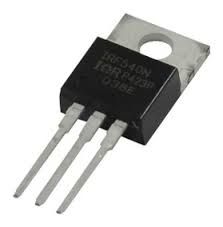
\includegraphics[scale=0.5]{2.jpeg}
\caption{El transistor MOSFET son de bajo costo y altas resistencia y capacidad}
\end{center}
\end{figure}

\section{Características técnicas de elementos activa dores}

La lista de \emph{"características ideales de trabajo de los transistores"} describe elementos activadores en condiciones ideales, pero ese es el problema que la mayoría de estos dispositivos semiconductores no trabaja en esas condiciones por lo cual, cada fabricante diseña una hoja de datos técnicos en los cuales da a conocer la forma de trabajar de cada dispositivo, la hoja esta determinada como \emph{\textbf{Datasheet}} la cual es propia del dispositivo, fabricante y encapsulado.

\newpage

Lo importante en esta sección sera el calculo de esas condiciones en las que debe trabajar un transistor para funcionar con un circuito, el cual esta dado por la siguientes características:

\begin{itemize}
\item Capacidades de voltaje
\item Capacidades de corriente
\item Velocidad o frecuencia de interrupción
\item 
\end{itemize}

De manera mas visual podemos observar en la figura 2 como es que diferentes tipos de transistores trabajan con sus capacidades máximas en cuanto voltajes y corrientes:

\begin{figure}[h]
\begin{center}
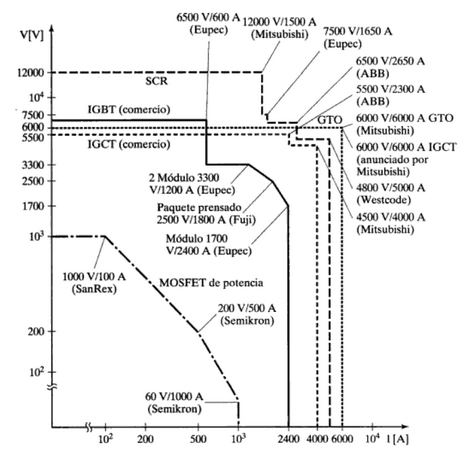
\includegraphics[scale=0.6]{3.png}
\caption{corrientes y tensiones con las que trabajan dispositivos de potencia}
\end{center}
\end{figure}

\section{Características de los dispositivos prácticos}

Estos tipos de transistores con conmutación trabajan con determinados tiempos, los cuales están definidos como los siguientes:

\begin{itemize}

\item un tiempo de demora
\item tiempo de subida
\item tiempo de almacenamiento
\item tiempo de bajada

\end{itemize}

\newpage

De manera tal que cuando la corriente satura y comienza con el tiempo de subida, de manera contraria el voltaje comenzara con su tiempo de bajada, y cuando la corriente trabaje en el tiempo de bajada el voltaje iniciara la subida, el tiempo de cerrado de un dispositivo es la suma del tiempo de retardo y el tiempo de subida, algo así como lo muestran la imagen 3:

\begin{figure}[h]
\begin{center}
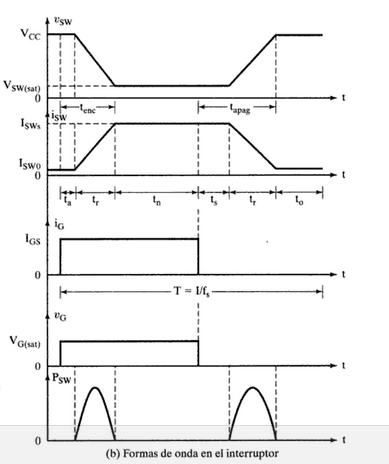
\includegraphics[scale=0.6]{4.png}
\caption{diferentes ondas con las que trabaja un transistor de potencia}
\end{center}
\end{figure}

La perdida promedio de potencia de potencia en la conducción $P_enc$ esta determinada por:

\begin{equation}
P_enc= \frac{1}{TS}\int p dt
\end{equation}

La perdida de conmutación que resulta, Psw durante los periodos de cerrado ya abierto se determina con:

\begin{figure}[h]
\begin{center}
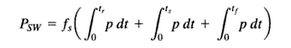
\includegraphics[scale=0.4]{5.png}
\end{center}
\end{figure}

Las especificaciones que debe de mantener son las siguientes:

\begin{itemize}
\item capacidades de voltaje: voltajes pico repetitivos directo e inverso y caída de voltaje den directo en el estado cerrado.
\item capacidades corriente: corrientes y promedio, raíces cuadráticas media.
\item velocidad o frecuencia de interrupción, cambio de un estado totalmente conductor hasta un estado totalmente no conductor, son parámetros muy importantes el periodo y la frecuencia de interrupción, que están dadas por:

\begin{center}

$F_s=\frac{1}{TS}=\frac{1}{t_d+t_e+t_r+t_s+t_f+t_a}$
\end{center}

\end{itemize}

\cite{rashid2004electronica}

\newpage

\bibliographystyle{apalike}
\bibliography{ref}

  


\end{document}